\usetikzlibrary{shapes.geometric, arrows.meta, positioning, calc}

\chapter{Esercizi PL}

\section{Totale Giugno 2026}
Dato il seguente schema, produrre
\begin{enumerate}
    \item prima una sua versione ottimizzata e semplificata, e
    \item poi la traduzione di tale versione nel modello relazionale, comprese le chiavi e i vincoli di integrità referenziale.
\end{enumerate}

Dato il seguente schema, produrre
\begin{enumerate}
    \item prima una sua versione ottimizzata e semplificata, e
    \item poi la traduzione di tale versione nel modello relazionale, comprese le chiavi e i vincoli di integrità referenziale.
\end{enumerate}

\begin{center}
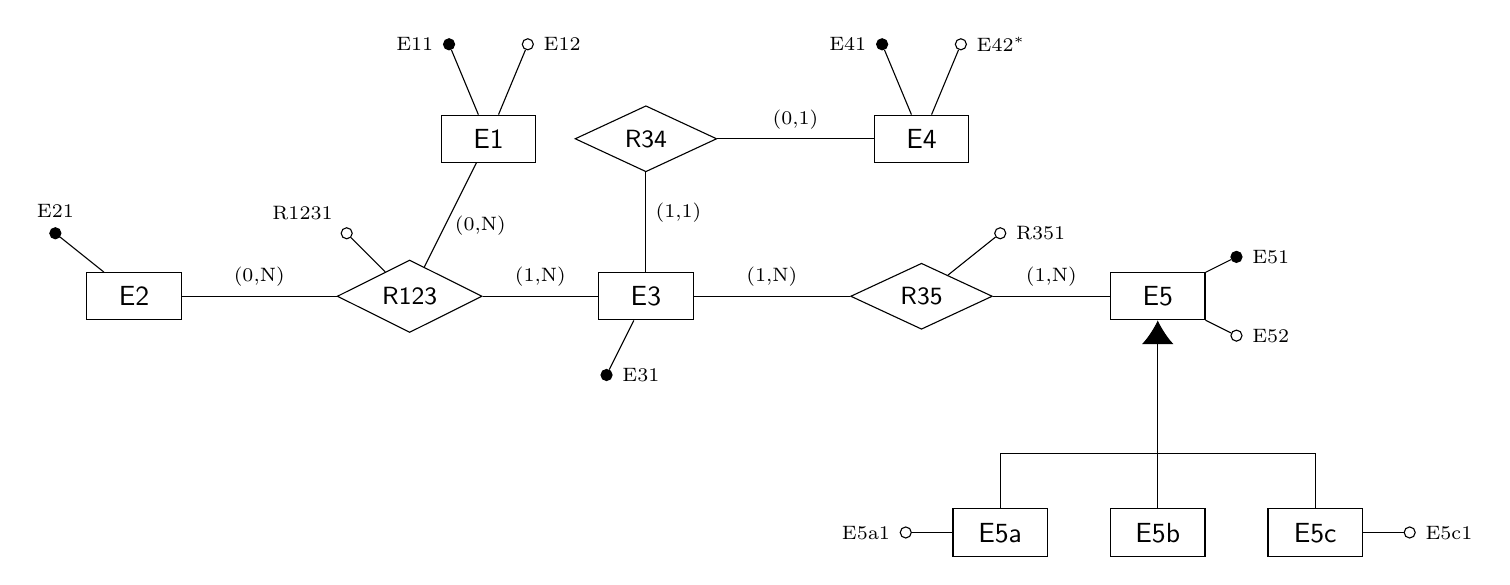
\begin{tikzpicture}[
    node distance=2cm,
    entity/.style={draw, rectangle, minimum width=1.2cm, minimum height=0.6cm, font=\sffamily},
    rel/.style={draw, diamond, aspect=2, minimum width=1.8cm, minimum height=0.6cm, font=\small\sffamily},
    attr/.style={draw, circle, inner sep=0pt, minimum size=4pt},
    key/.style={draw, circle, fill=black, inner sep=0pt, minimum size=4pt},
    label text/.style={font=\scriptsize}
]

% Entities
\node[entity] (E1) at (0, 3) {E1};
\node[entity] (E2) at (-4.5, 1) {E2};
\node[entity] (E3) at (2, 1) {E3};
\node[entity] (E4) at (5.5, 3) {E4};
\node[entity] (E5) at (8.5, 1) {E5};

\node[entity] (E5a) at (6.5, -2) {E5a};
\node[entity] (E5b) at (8.5, -2) {E5b};
\node[entity] (E5c) at (10.5, -2) {E5c};

% Relationships
\node[rel] (R123) at (-1, 1) {R123};
\node[rel] (R34)  at (2, 3) {R34};
\node[rel] (R35)  at (5.5, 1) {R35};

% Attributes for E1
\node[key, label={[label text]left:E11}] (E11) at (-0.5, 4.2) {};
\node[attr, label={[label text]right:E12}] (E12) at (0.5, 4.2) {};
\draw (E1) -- (E11);
\draw (E1) -- (E12);

% Attributes for E2
\node[key, label={[label text]above:E21}] (E21) at (-5.5, 1.8) {};
\draw (E2) -- (E21);

% Attributes for E3
\node[key, label={[label text]right:E31}] (E31) at (1.5, 0) {};
\draw (E3) -- (E31);

% Attributes for E4
\node[key, label={[label text]left:E41}] (E41) at (5, 4.2) {};
\node[attr, label={[label text]right:E42$^*$}] (E42) at (6, 4.2) {};
\draw (E4) -- (E41);
\draw (E4) -- (E42);

% Attributes for E5
\node[key, label={[label text]right:E51}] (E51) at (9.5, 1.5) {};
\node[attr, label={[label text]right:E52}] (E52) at (9.5, 0.5) {};
\draw (E5) -- (E51);
\draw (E5) -- (E52);

% Attributes for R123
\node[attr, label={[label text]above left:R1231}] (R1231) at (-1.8, 1.8) {};
\draw (R123) -- (R1231);

% Attributes for R35
\node[attr, label={[label text]right:R351}] (R351) at (6.5, 1.8) {};
\draw (R35) -- (R351);

% Attributes for Children
\node[attr, label={[label text]left:E5a1}] (E5a1) at (5.3, -2) {};
\draw (E5a) -- (E5a1);
\node[attr, label={[label text]right:E5c1}] (E5c1) at (11.7, -2) {};
\draw (E5c) -- (E5c1);

% Links Entity-Relationship
\draw (E1) -- node[right, font=\scriptsize, pos=0.6] {(0,N)} (R123);
\draw (E2) -- node[above, font=\scriptsize] {(0,N)} (R123);
\draw (E3) -- node[above, font=\scriptsize] {(1,N)} (R123);

\draw (E3) -- node[right, font=\scriptsize, pos=0.6] {(1,1)} (R34);
\draw (E4) -- node[above, font=\scriptsize] {(0,1)} (R34);

\draw (E3) -- node[above, font=\scriptsize] {(1,N)} (R35);
\draw (E5) -- node[above, font=\scriptsize] {(1,N)} (R35);

% Generalization
\draw (E5a.north) -- +(0, 0.7) coordinate (A);
\draw (E5b.north) -- +(0, 0.7) coordinate (B);
\draw (E5c.north) -- +(0, 0.7) coordinate (C);
\draw (A) -- (C);
\draw[-{Latex[length=3mm, width=4mm]}] (B) -- (E5.south);

\end{tikzpicture}
\end{center}

\subsection{Semplificazione ER}
\begin{center}
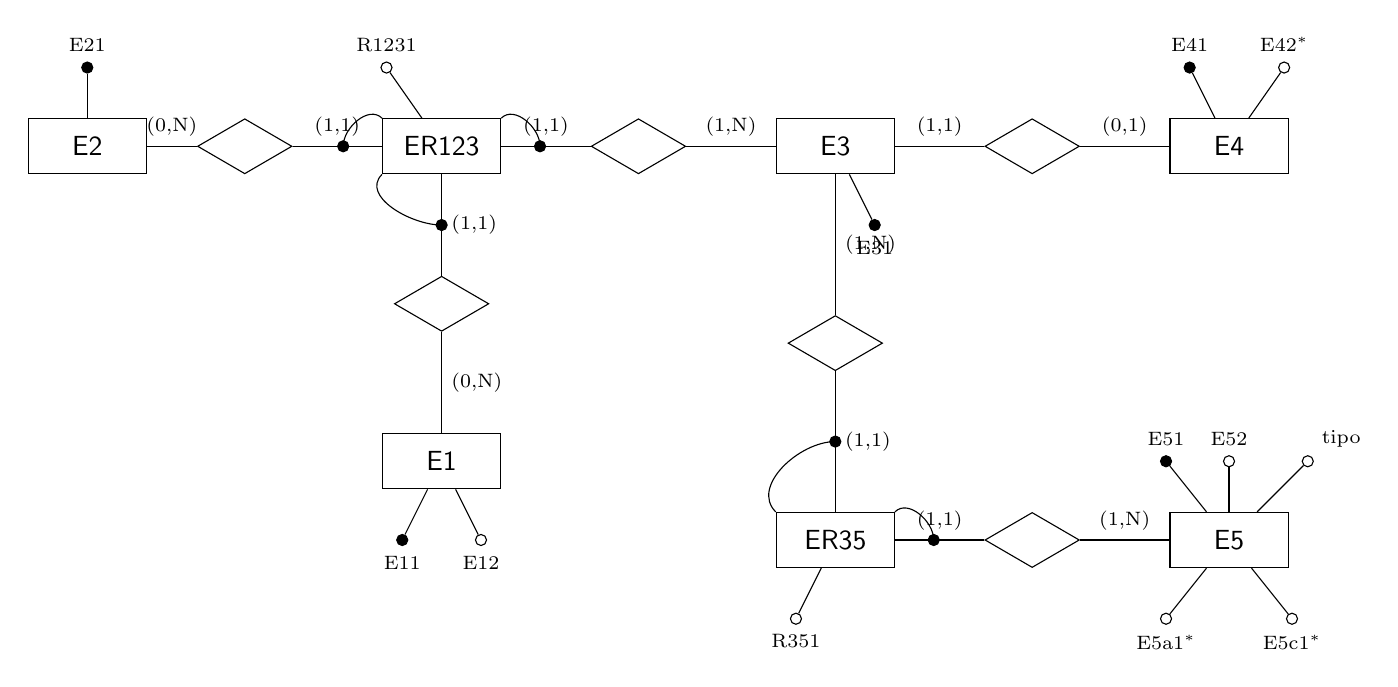
\begin{tikzpicture}[
    node distance=2cm,
    entity/.style={draw, rectangle, minimum width=1.5cm, minimum height=0.7cm, font=\sffamily},
    rel/.style={draw, diamond, aspect=1.5, minimum width=1.2cm, minimum height=0.7cm, font=\small\sffamily},
    attr/.style={draw, circle, inner sep=0pt, minimum size=4pt},
    key/.style={draw, circle, fill=black, inner sep=0pt, minimum size=4pt},
    label text/.style={font=\scriptsize}
]

% Nodes
\node[entity] (E2) at (0, 0) {E2};
\node[rel] (R_E2_ER123) at (2, 0) {};
\node[entity] (ER123) at (4.5, 0) {ER123};
\node[rel] (R_E1_ER123) at (4.5, -2) {};
\node[entity] (E1) at (4.5, -4) {E1};
\node[rel] (R_E3_ER123) at (7, 0) {};
\node[entity] (E3) at (9.5, 0) {E3};
\node[rel] (R_E3_E4) at (12, 0) {};
\node[entity] (E4) at (14.5, 0) {E4};

\node[rel] (R_E3_ER35) at (9.5, -2.5) {};
\node[entity] (ER35) at (9.5, -5) {ER35};
\node[rel] (R_E5_ER35) at (12, -5) {};
\node[entity] (E5) at (14.5, -5) {E5};

% Attributes E2
\node[key, label={[label text]above:E21}] (E21) at (0, 1) {};
\draw (E2) -- (E21);

% Attributes ER123
\node[attr, label={[label text]above:R1231}] (R1231) at (3.8, 1) {};
\draw (ER123) -- (R1231);

% Attributes E1
\node[key, label={[label text]below:E11}] (E11) at (4, -5) {};
\node[attr, label={[label text]below:E12}] (E12) at (5, -5) {};
\draw (E1) -- (E11);
\draw (E1) -- (E12);

% Attributes E3
\node[key, label={[label text]below:E31}] (E31) at (10, -1) {};
\draw (E3) -- (E31);

% Attributes E4
\node[key, label={[label text]above:E41}] (E41) at (14, 1) {};
\node[attr, label={[label text]above:E42$^*$}] (E42) at (15.2, 1) {};
\draw (E4) -- (E41);
\draw (E4) -- (E42);

% Attributes ER35
\node[attr, label={[label text]below:R351}] (R351) at (9, -6) {};
\draw (ER35) -- (R351);

% Attributes E5
\node[key, label={[label text]above:E51}] (E51) at (13.7, -4) {};
\node[attr, label={[label text]above:E52}] (E52) at (14.5, -4) {};
\node[attr, label={[label text]above right:tipo}] (tipo) at (15.5, -4) {};
\node[attr, label={[label text]below:E5a1$^*$}] (E5a1) at (13.7, -6) {};
\node[attr, label={[label text]below:E5c1$^*$}] (E5c1) at (15.3, -6) {};
\draw (E5) -- (E51);
\draw (E5) -- (E52);
\draw (E5) -- (tipo);
\draw (E5) -- (E5a1);
\draw (E5) -- (E5c1);

% Relationships Edges
\draw (E2) -- node[above, font=\scriptsize] {(0,N)} (R_E2_ER123);
\draw (R_E2_ER123) -- node[above, font=\scriptsize] {(1,1)} (ER123);

\draw (E1) -- node[right, font=\scriptsize] {(0,N)} (R_E1_ER123);
\draw (R_E1_ER123) -- node[right, font=\scriptsize] {(1,1)} (ER123);

\draw (E3) -- node[above, font=\scriptsize] {(1,N)} (R_E3_ER123);
\draw (R_E3_ER123) -- node[above, font=\scriptsize] {(1,1)} (ER123);

\draw (E3) -- node[above, font=\scriptsize] {(1,1)} (R_E3_E4);
\draw (R_E3_E4) -- node[above, font=\scriptsize] {(0,1)} (E4);

\draw (E3) -- node[right, font=\scriptsize] {(1,N)} (R_E3_ER35);
\draw (R_E3_ER35) -- node[right, font=\scriptsize] {(1,1)} (ER35);

\draw (E5) -- node[above, font=\scriptsize] {(1,N)} (R_E5_ER35);
\draw (R_E5_ER35) -- node[above, font=\scriptsize] {(1,1)} (ER35);

% External Identifiers (arcs with dots representing the weak entity dependencies)
\draw (ER123.north west) to[out=135, in=90] (3.25, 0) node[key, inner sep=0.8pt] {};
\draw (ER123.south west) to[out=225, in=180] (4.5, -1) node[key, inner sep=0.8pt] {};
\draw (ER123.north east) to[out=45, in=90] (5.75, 0) node[key, inner sep=0.8pt] {};

\draw (ER35.north west) to[out=135, in=180] (9.5, -3.75) node[key, inner sep=0.8pt] {};
\draw (ER35.north east) to[out=45, in=90] (10.75, -5) node[key, inner sep=0.8pt] {};

\end{tikzpicture}
\end{center}

\subsection{Trasformazione in MR}
\begin{itemize}
    \item E2(\underline{E21})
    \item E1(\underline{E11}, E12)
    \item E3(\underline{E31}, E41)
    \item E4(\underline{E41}, $E42^*$)
    \item E5(\underline{E51}, E52, tipo, $E5a1^*, E5c1^*$)
    \item ER123(\underline{E21, E11, E31}, R1231)
    \item ER35(\underline{E31, E51}, R351)
\end{itemize}

\newpage
\section{Es 1}
Sia dato lo schema concettuale in figura, dove gli attributi e gli identificatori delle entità sono rappresentati a lato delle relative entità. Si supponga che il carico applicativo (interrogazioni + transazioni di aggiornamento) sia tale che le entità B, C, e D vengano con grande frequenza accedute tutte insieme.
\begin{enumerate}
    \item Tradurre lo schema concettuale in un nuovo schema in cui siano eliminate le strutture non direttamente traducibili nel modello relazionale.
    \item Tradurre il nuovo schema nel modello relazionale.
\end{enumerate}

\vspace{1.5cm}

\begin{center}
\begin{tikzpicture}[
    node distance=2cm,
    entity/.style={draw, rectangle, minimum width=1.5cm, minimum height=0.7cm, font=\sffamily},
    rel/.style={draw, diamond, aspect=2, minimum width=1.8cm, minimum height=0.6cm, font=\small\sffamily},
    attr/.style={draw, circle, inner sep=0pt, minimum size=4pt},
    key/.style={draw, circle, fill=black, inner sep=0pt, minimum size=4pt},
    label text/.style={font=\scriptsize}
]

% Nodes
\node[entity] (B) at (0, 0) {B};
\node[entity] (A) at (6, 0) {A};

\node[rel] (R2AB) at (3, 1.2) {R2AB};
\node[rel] (R1AB) at (3, -1.2) {R1AB};

\node[entity] (C) at (-2.5, -3.5) {C};
\node[rel] (RCD) at (0, -3.5) {RCD};
\node[entity] (D) at (2.5, -3.5) {D};

\node[rel] (RAEF) at (6, -3.5) {RAEF};
\node[entity] (E) at (10, -3.5) {E};
\node[entity] (F) at (6, -6.5) {F};

% Attributes B
\node[key, label={[label text]left:KB}] (KB) at (-1, 0.5) {};
\node[attr, label={[label text]left:B1}] (B1) at (-1, -0.2) {};
\draw (B) -- (KB);
\draw (B) -- (B1);

% Attributes A
\node[key, label={[label text]right:KA}] (KA) at (7, 0.5) {};
\node[attr, label={[label text]right:A1}] (A1) at (7, -0.2) {};
\draw (A) -- (KA);
\draw (A) -- (A1);

% Attributes C
\node[attr, label={[label text]left:C1}] (C1) at (-3.5, -3) {};
\node[attr, label={[label text]left:C2}] (C2) at (-3.5, -4) {};
\draw (C) -- (C1);
\draw (C) -- (C2);

% Attributes D
\node[attr, label={[label text]right:D1}] (D1) at (3.5, -3) {};
\node[attr, label={[label text]right:D2}] (D2) at (3.5, -4) {};
\draw (D) -- (D1);
\draw (D) -- (D2);

% Attributes E
\node[key, label={[label text]right:KE}] (KE) at (11, -3) {};
\node[attr, label={[label text]right:E1}] (E1) at (11, -4) {};
\draw (E) -- (KE);
\draw (E) -- (E1);

% Attributes F
\node[key, label={[label text]right:KF}] (KF) at (7, -6) {};
\node[attr, label={[label text]right:F1}] (F1) at (7, -7) {};
\draw (F) -- (KF);
\draw (F) -- (F1);

% Attribute RAEF
\node[attr, label={[label text]right:G}] (G) at (7.2, -2.5) {};
\draw (RAEF) -- (G);

% Relationships B-A
\draw (B) -- node[above left, font=\scriptsize] {(0,1)} (R2AB);
\draw (R2AB) -- node[above right, font=\scriptsize] {(1,1)} (A);

\draw (B) -- node[below left, font=\scriptsize] {(1,n)} (R1AB);
\draw (R1AB) -- node[below right, font=\scriptsize] {(1,1)} (A);

% Relationships C-D
\draw (C) -- node[above, font=\scriptsize] {(1,n)} (RCD);
\draw (RCD) -- node[above, font=\scriptsize] {(1,n)} (D);

% Relationships RAEF
\draw (A) -- node[right, font=\scriptsize] {(1,n)} (RAEF);
\draw (RAEF) -- node[above, font=\scriptsize] {(1,n)} (E);
\draw (RAEF) -- node[left, font=\scriptsize] {(1,n)} (F);

% Generalization
\draw (C.north) -- +(0, 1) coordinate (C_up);
\draw (D.north) -- +(0, 1) coordinate (D_up);
\draw (C_up) -- (D_up);
\draw[-{Latex[length=3mm, width=4mm]}] ($(C_up)!0.5!(D_up)$) -- (B.south);

\end{tikzpicture}
\end{center}

\subsection{Semplificazione ER}
\begin{center}
\begin{tikzpicture}[
    node distance=2cm,
    entity/.style={draw, rectangle, minimum width=1.5cm, minimum height=0.7cm, font=\sffamily},
    rel/.style={draw, diamond, aspect=1.5, minimum width=1.2cm, minimum height=0.7cm, font=\small\sffamily},
    attr/.style={draw, circle, inner sep=0pt, minimum size=4pt},
    key/.style={draw, circle, fill=black, inner sep=0pt, minimum size=4pt},
    label text/.style={font=\scriptsize}
]

% ====================
% Nodi Principali
% ====================
\node[entity, minimum width=2.2cm] (B) at (0, 0) {B};
\node[entity] (A) at (7, 0) {A};

% Relazioni tra B e A
\node[rel] (R2AB) at (3.5, 1.5) {};
\node[rel] (R1AB) at (3.5, -1.5) {};

% Relazione Ricorsiva RCD
\node[rel] (RCD_L) at (-2, -3.5) {};
\node[rel] (RCD_R) at (2, -3.5) {};
\node[entity] (RCD) at (0, -7) {RCD};

% Relazione RAEF
\node[rel] (RA_RAEF) at (7, -2.5) {};
\node[entity] (RAEF) at (7, -5) {RAEF};
\node[rel] (RRAEF_E) at (10, -5) {};
\node[entity] (E) at (13, -5) {E};
\node[rel] (RRAEF_F) at (7, -7.5) {};
\node[entity] (F) at (7, -10) {F};

% ====================
% Attributi
% ====================
% Attributi di B
\node[attr, label={[label text]left:D1$^*$}] (D1) at (-1.7, 0.3) {};
\node[attr, label={[label text]left:D2$^*$}] (D2) at (-1.7, -0.3) {};
\node[attr, label={[label text]above left:C2$^*$}] (C2) at (-1, 1) {};
\node[attr, label={[label text]above:C1$^*$}] (C1) at (-0.3, 1) {};
\node[attr, label={[label text]above:tipo}] (tipo) at (0.4, 1) {};
\node[key, label={[label text]above:KB}] (KB) at (1.1, 1) {};
\node[attr, label={[label text]above right:B1}] (B1) at (1.6, 0.6) {};
\draw (B) -- (D1); \draw (B) -- (D2); \draw (B) -- (C2); \draw (B) -- (C1);
\draw (B) -- (tipo); \draw (B) -- (KB); \draw (B) -- (B1);

% Attributi di A
\node[key, label={[label text]right:KA}] (KA) at (8, 0.3) {};
\node[attr, label={[label text]right:A1}] (A1) at (8, -0.3) {};
\draw (A) -- (KA); \draw (A) -- (A1);

% Attributi di E
\node[key, label={[label text]right:KE}] (KE) at (14, -4.7) {};
\node[attr, label={[label text]right:E1}] (E1) at (14, -5.3) {};
\draw (E) -- (KE); \draw (E) -- (E1);

% Attributi di F
\node[key, label={[label text]below:KF}] (KF) at (6.5, -11) {};
\node[attr, label={[label text]below:F1}] (F1) at (7.5, -11) {};
\draw (F) -- (KF); \draw (F) -- (F1);

% Attributo di RAEF
\node[attr, label={[label text]left:G}] (G) at (5.5, -5) {};
\draw (RAEF) -- (G);

% ====================
% Collegamenti e Cardinalità
% ====================
% B <-> A
\draw (B) -- node[above left, font=\scriptsize] {(0,1)} (R2AB);
\draw (R2AB) -- node[above right, font=\scriptsize] {(1,1)} (A);

\draw (B) -- node[below left, font=\scriptsize] {(1,n)} (R1AB);
\draw (R1AB) -- node[below right, font=\scriptsize] {(1,1)} (A);

% B <-> RCD
\draw (B) -- node[left=0.2cm, font=\scriptsize] {(0,N)} (RCD_L);
\draw (RCD_L) -- node[left, font=\scriptsize] {(1,1)} (RCD);

\draw (B) -- node[right=0.2cm, font=\scriptsize] {(0,N)} (RCD_R);
\draw (RCD_R) -- node[right, font=\scriptsize] {(1,1)} (RCD);

% RAEF
\draw (A) -- node[right, font=\scriptsize] {(1,N)} (RA_RAEF);
\draw (RA_RAEF) -- node[right, font=\scriptsize] {(1,1)} (RAEF);

\draw (RAEF) -- node[above, font=\scriptsize] {(1,1)} (RRAEF_E);
\draw (RRAEF_E) -- node[above, font=\scriptsize] {(1,N)} (E);

\draw (RAEF) -- node[right, font=\scriptsize] {(1,1)} (RRAEF_F);
\draw (RRAEF_F) -- node[right, font=\scriptsize] {(1,N)} (F);

% ====================
% Identificatori Esterni (Archetti con pallino)
% ====================
% Archetto per RCD
\coordinate (P_RCD_L) at ($(RCD_L)!0.4!(RCD)$);
\coordinate (P_RCD_R) at ($(RCD_R)!0.4!(RCD)$);
\draw (P_RCD_L) node[key, inner sep=1.2pt] {} to[out=-45, in=225] (P_RCD_R);

% Archetto per RAEF
\coordinate (P_RAEF_T) at ($(RA_RAEF)!0.5!(RAEF)$);
\coordinate (P_RAEF_R) at ($(RAEF)!0.5!(RRAEF_E)$);
\coordinate (P_RAEF_B) at ($(RAEF)!0.5!(RRAEF_F)$);

\draw (P_RAEF_T) node[key, inner sep=1.2pt] {} 
      to[out=0, in=90] (8.5, -5) 
      to[out=-90, in=0] (P_RAEF_B);

\end{tikzpicture}
\end{center}

\subsection{Traduzione in MR}
\begin{itemize}
    \item A(\underline{KA}, KB\_1, KB\_2, A1)
    \item B(\underline{KB}, B1, tipo, $C1^*, C2^*, D1^*, D2^*$)
    \item E(\underline{KE}, E1)
    \item F(\underline{KF}, F1)
    \item RCD(\underline{KB\_C, KB\_D})
    \item RAEF(\underline{KF, KE, KA}, G)
\end{itemize}

\newpage
\section{Es 2}
\noindent Dato lo schema ER in figura, in cui gli attributi di entità e relazioni sono collocati accanto all'entità o alla relazione e gli identificatori sono sottolineati:

\begin{enumerate}
    \item Tradurlo in un nuovo schema in cui siano eliminate le strutture non direttamente traducibili in uno schema relazionale (e disegnarlo).
    \item Tradurre il nuovo schema nel modello relazionale.
\end{enumerate}

\vspace{1cm}

\begin{center}
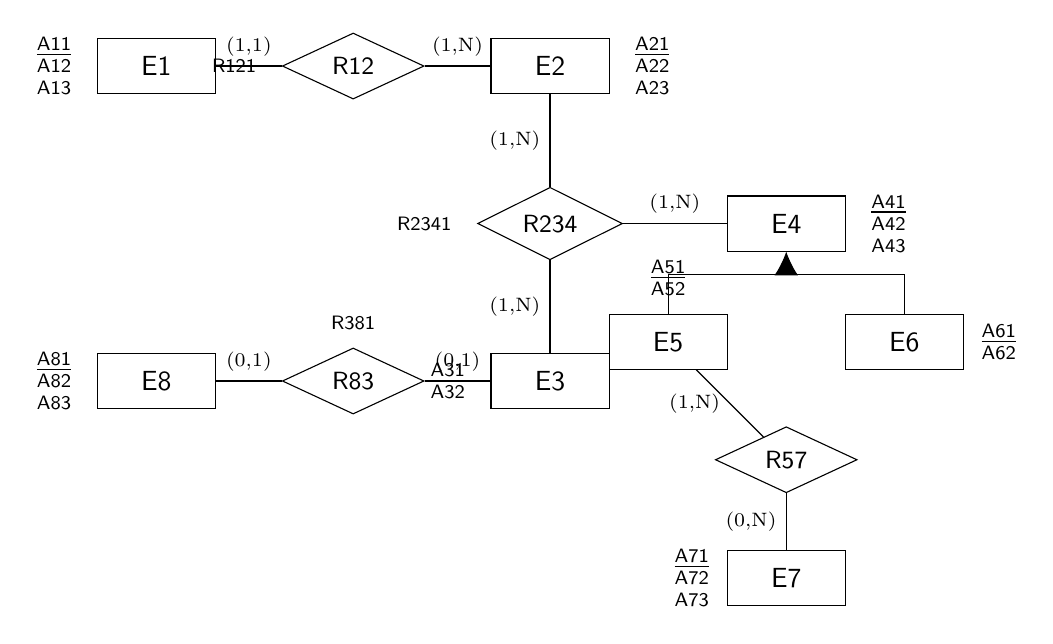
\begin{tikzpicture}[
    node distance=2cm,
    entity/.style={draw, rectangle, minimum width=1.5cm, minimum height=0.7cm, font=\sffamily},
    rel/.style={draw, diamond, aspect=2, minimum width=1.8cm, minimum height=0.6cm, font=\small\sffamily},
    attr_container/.style={align=left, font=\scriptsize\sffamily},
    label text/.style={font=\scriptsize}
]

% Nodes
\node[entity] (E1) at (0, 0) {E1};
\node[rel] (R12) at (2.5, 0) {R12};
\node[entity] (E2) at (5, 0) {E2};
\node[rel] (R234) at (5, -2) {R234};
\node[entity] (E4) at (8, -2) {E4};
\node[entity] (E3) at (5, -4) {E3};
\node[rel] (R83) at (2.5, -4) {R83};
\node[entity] (E8) at (0, -4) {E8};

\node[entity] (E5) at (6.5, -3.5) {E5};
\node[entity] (E6) at (9.5, -3.5) {E6};
\node[rel] (R57) at (8, -5) {R57};
\node[entity] (E7) at (8, -6.5) {E7};

% Attributes (Text next to entities/rels)
\node[left=0.2cm of E1, attr_container] {\underline{A11}\\A12\\A13};
\node[right=0.2cm of E2, attr_container] {\underline{A21}\\A22\\A23};
\node[left=0.2cm of R12, attr_container] {R121};
\node[left=0.2cm of R234, attr_container] {R2341};
\node[right=0.2cm of E4, attr_container] {\underline{A41}\\A42\\A43};
\node[left=0.2cm of E3, attr_container] {\underline{A31}\\A32};
\node[left=0.2cm of E8, attr_container] {\underline{A81}\\A82\\A83};
\node[above=0.1cm of R83, attr_container] {R381};
\node[above=0.1cm of E5, attr_container] {\underline{A51}\\A52};
\node[right=0.1cm of E6, attr_container] {\underline{A61}\\A62};
\node[left=0.1cm of E7, attr_container] {\underline{A71}\\A72\\A73};

% Relationships Edges
\draw (E1) -- node[above, label text] {(1,1)} (R12);
\draw (R12) -- node[above, label text] {(1,N)} (E2);

\draw (E2) -- node[left, label text] {(1,N)} (R234);
\draw (R234) -- node[above, label text] {(1,N)} (E4);
\draw (R234) -- node[left, label text] {(1,N)} (E3);

\draw (E8) -- node[above, label text] {(0,1)} (R83);
\draw (R83) -- node[above, label text] {(0,1)} (E3);

\draw (E5) -- node[left, label text] {(1,N)} (R57);
\draw (R57) -- node[left, label text] {(0,N)} (E7);

% Generalization
\draw (E5.north) -- ++(0, 0.5) coordinate (E5_up);
\draw (E6.north) -- ++(0, 0.5) coordinate (E6_up);
\draw (E5_up) -- (E6_up);
\draw[-{Latex[length=3mm, width=3mm]}] ($(E5_up)!0.5!(E6_up)$) -- (E4.south);

\end{tikzpicture}
\end{center}

\subsection{Semplificazione ER}
\begin{center}
\begin{tikzpicture}[
    node distance=1.8cm,
    entity/.style={draw, rectangle, minimum width=1.2cm, minimum height=0.6cm, font=\sffamily\small},
    rel/.style={draw, diamond, aspect=1.5, minimum width=1cm, minimum height=0.5cm, font=\tiny\sffamily},
    attr/.style={draw, circle, inner sep=0pt, minimum size=3pt},
    key/.style={draw, circle, fill=black, inner sep=0pt, minimum size=3pt},
    label text/.style={font=\tiny}
]

% Nodes
\node[entity] (E1) at (0, 0) {E1};
\node[rel] (R12) at (1.8, 0) {};
\node[entity] (E2) at (3.6, 0) {E2};

\node[rel] (R234_rel) at (3.6, -1.2) {};
\node[entity, minimum width=2.5cm] (R234) at (3.6, -2.4) {R234};
\node[rel] (R234_r) at (5.5, -2.4) {};
\node[entity] (E4) at (7.5, -2.4) {E4};

\node[rel] (R234_e3) at (3.6, -3.6) {};
\node[entity] (E3) at (3.6, -4.8) {E3};

\node[rel] (R83_r) at (1.8, -4.8) {};
\node[entity] (E8) at (0, -4.8) {E8};

\node[rel] (E4_E5) at (7.5, -3.6) {};
\node[entity] (E5) at (7.5, -4.8) {E5};
\node[rel] (R57_rel) at (7.5, -6) {};
\node[entity, minimum width=1.5cm] (R57) at (7.5, -7.2) {R57};
\node[rel] (R57_e7) at (7.5, -8.4) {};
\node[entity] (E7) at (7.5, -9.6) {E7};

\node[rel] (E4_E6) at (9.5, -2.4) {};
\node[entity] (E6) at (9.5, -3.6) {E6};

% Attributi E1
\node[key, label={[label text]above:A11}] (A11) at (-0.5, 0.7) {};
\node[attr, label={[label text]left:A12}] (A12) at (-0.8, 0) {};
\node[attr, label={[label text]below:A13}] (A13) at (-0.5, -0.7) {};
\draw (E1) -- (A11); \draw (E1) -- (A12); \draw (E1) -- (A13);

% Attributi E2
\node[key, label={[label text]above:A21}] (A21) at (3.1, 0.7) {};
\node[attr, label={[label text]above:A22}] (A22) at (3.8, 0.7) {};
\node[attr, label={[label text]right:A23}] (A23) at (4.5, 0.7) {};
\draw (E2) -- (A21); \draw (E2) -- (A22); \draw (E2) -- (A23);

% Attributi E8
\node[key, label={[label text]above:A81}] (A81) at (-0.5, -5.5) {};
\node[attr, label={[label text]above:A82}] (A82) at (0, -5.5) {};
\node[attr, label={[label text]below:A83}] (A83) at (-0.5, -6.2) {};
\draw (E8) -- (A81); \draw (E8) -- (A82); \draw (E8) -- (A83);

% Attributi E3
\node[key, label={[label text]below:A31}] (A31) at (3.2, -5.5) {};
\node[attr, label={[label text]right:A32}] (A32) at (4.0, -5.5) {};
\draw (E3) -- (A31); \draw (E3) -- (A32);

% Attributi E4
\node[key, label={[label text]above:A41}] (A41) at (7, -3.1) {};
\node[attr, label={[label text]above:A42}] (A42) at (7.5, -3.1) {};
\node[attr, label={[label text]right:A43}] (A43) at (8.1, -2.4) {};
\draw (E4) -- (A41); \draw (E4) -- (A42); \draw (E4) -- (A43);

% Attributi E5
\node[attr, label={[label text]left:A51}] (A51) at (7, -4.8) {};
\node[attr, label={[label text]left:A52}] (A52) at (7, -5.4) {};
\draw (E5) -- (A51); \draw (E5) -- (A52);

% Attributi E6
\node[key, label={[label text]below:A61}] (A61) at (9.2, -4.3) {};
\node[attr, label={[label text]below:A62}] (A62) at (9.8, -4.3) {};
\draw (E6) -- (A61); \draw (E6) -- (A62);

% Attributi E7
\node[key, label={[label text]below:A71}] (A71) at (7, -10.3) {};
\node[attr, label={[label text]below:A72}] (A72) at (7.5, -10.3) {};
\node[attr, label={[label text]below:A73}] (A73) at (8, -10.3) {};
\draw (E7) -- (A71); \draw (E7) -- (A72); \draw (E7) -- (A73);

% Collegamenti
\draw (E1) -- node[label text, above] {(1,1)} (R12);
\draw (R12) -- node[label text, above] {(1,N)} (E2);

\draw (E2) -- node[label text, left] {(1,N)} (R234_rel);
\draw (R234_rel) -- (R234);
\draw (R234) -- (R234_r) -- (E4) node[midway, label text, above] {(1,N)};
\draw (R234) -- (R234_e3) -- (E3) node[midway, label text, left] {(1,N)};

\draw (E8) -- (R83_r) -- (E3) node[midway, label text, above] {(0,1)};

\draw (E4) -- (E4_E5) -- (E5) node[midway, label text, right] {(0,1)};
\draw (E4) -- (E4_E6) -- (E6) node[midway, label text, right] {(1,1)};

\draw (E5) -- (R57_rel) -- (R57);
\draw (R57) -- (R57_e7) -- (E7) node[midway, label text, right] {(0,N)};

% Identificatori
\draw (E1.north) to[out=110, in=180] (A11) node[key, inner sep=0.7pt] {};
\draw (R234.north west) to[out=135, in=90] (2.9, -2.4) node[key, inner sep=0.7pt] {};
\draw (R234.south west) to[out=225, in=180] (3.6, -3.1) node[key, inner sep=0.7pt] {};
\draw (R57.north west) to[out=135, in=180] (7.5, -6.5) node[key, inner sep=0.7pt] {};

\end{tikzpicture}
\end{center}

\subsection{Traduzione in MR}
\begin{itemize}
    \item E1(\underline{A11}, A21, A12, A13)
    \item E2(\underline{A21}, A22, A23)
    \item E3(\underline{A31}, A32)
    \item E4(\underline{A41}, A42, A43)
    \item E5(\underline{A51}, A41, A52)
    \item E6(\underline{A61}, A41, A62)
    \item E7(\underline{A71}, A72, A73)
    \item E8(\underline{A81}, A31, A82, A83)
    \item R234(\underline{A21, A31, A41})
    \item R57(\underline{A51, A71})
\end{itemize}